\chapter{Ein Überblick über Clusteranalyseverfahren}

Nach \citet[S. 476]{Backhaus.2016} lassen sich vier übergeordnete Gruppierungen von Clusteranalyseverfahren darstellen. Abbildung \ref{pic:backhaus476} gibt hierzu nochmal einen Überblick.

\begin{enumerate}
	\item Partitionierende Verfahren: Diese Algorithmen benötigen eine vorgegebene Clusteranzahl, in die sie die Objekte einzuordnen versuchen. Unterschiede zwischen den einzelnen Verfahren entstehen hierbei vor allem durch die unterschiedliche Messung der Verbesserung der Clusterbildung und in der Regelung des Austauschs der Objekte zwischen den Clustern.
	\item Hierarchische Verfahren: Im Gegensatz zu partitionierenden Verfahren benötigen diese Algorithmen keine vorgegebene Clusteranzahl, sondern iterieren alle möglichen Clusteranzahlen durch. Hierarchisch divisive Verfahren gehen dabei von der größtmöglichen Partition aus, die sie Schritt für Schritt in die kleinstmöglichen Partitionen zerlegen (ein Objekt in einer Partition). Hierarchisch agglomerative Verfahren dagegen fassen die feinsten Partitionen zu immer größeren Gruppen zusammen, bis schließlich die größtmögliche Partition erreicht ist, die alle Objekte enthält. Abbildung \ref{pic:xu21} zeigt diesen Unterschied deutlich.
	\begin{figure}[h]
		\begin{center}
			\includegraphics[width=8cm]{pics/xu21.png}
		\end{center}
		\caption{Vergleich der agglomerativen und divisiven Strategien nach Xu}
		\label{pic:xu21}
	\end{figure}
	\item Graphentheoretische Verfahren
	\item Optimierungsverfahren
\end{enumerate}

\begin{figure}[h]
	\begin{center}
		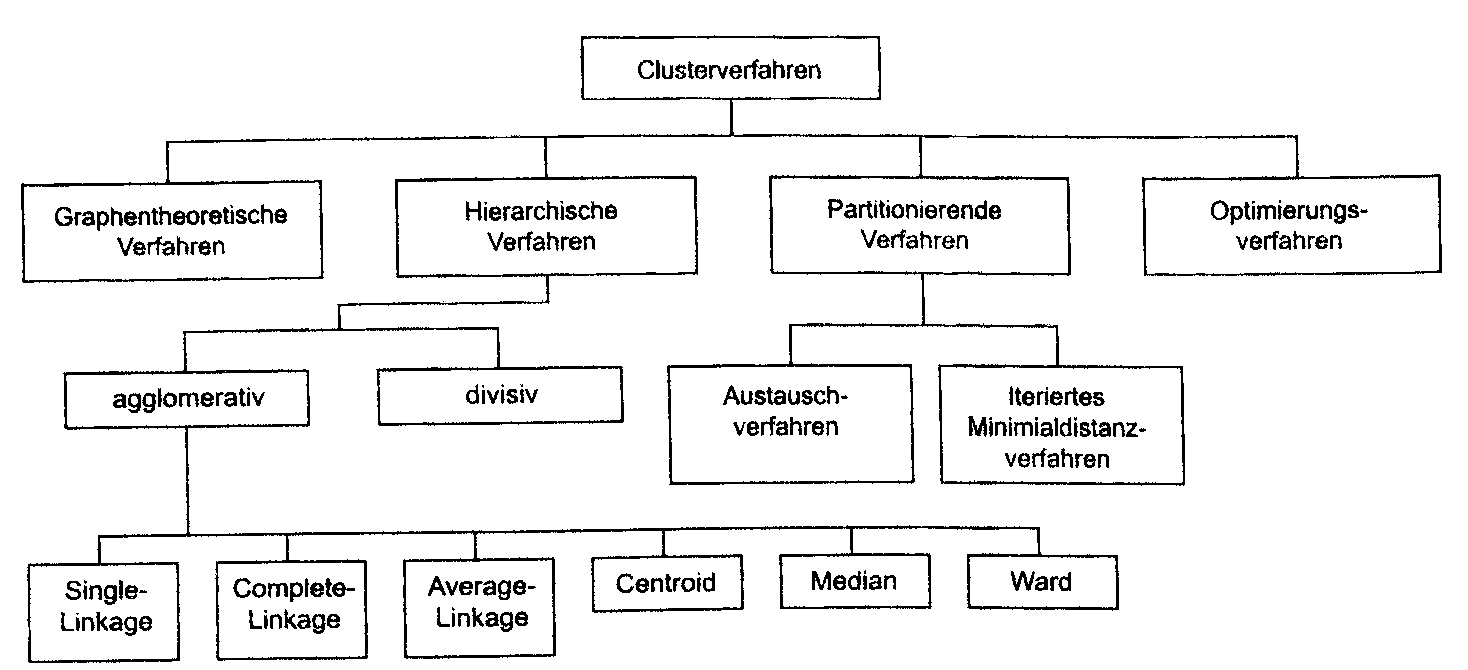
\includegraphics[width=14cm]{pics/backhaus476.png}
	\end{center}
	\caption{Gruppierungen nach Backhaus}
	\label{pic:backhaus476}
\end{figure}

\citet[S. 18]{Bacher.2010} unterscheiden andere Clusteranalyseverfahren auf Grundlage der Zuordnung der Klassifikationsobjekte zu den Clustern:

\begin{enumerate}
	\item Unvollständige Clusteranalyseverfahren: auch geometrische Methoden, Repräsentations- oder Projektverfahren, führen nur zu einer räumlichen Darstellung, nur bis dreidimensionalen Raum möglich
	\item Deterministische Clusteranalyseverfahren: Klassifikationsobjekte werden mit Wahrscheinlichkeit 1 einem oder mehreren Clustern zugeordnet, 
	\item Probabilistische Clusteranalyseverfahren: Fuzzy, Klassifikationsobjekte werden verschiedenen Clustern mit einer Wahrscheinlichkeit zwischen 0 und 1 zugeordnet, Verallgemeinerung der Deterministischen Clusteranalyseverfahren (Annahme, dass w = 0 oder 1 wird fallen gelassen)
\end{enumerate}

\citet[S. 21]{Bacher.2010} unterscheiden die Verfahren weiterhin auch aufgrund ihres zugrundeliegenden Wahrscheinlichkeitsmodells. Abbildung \ref{pic:bac20} beschreibt, welche Modelle welche Modelle zu welcher Zuordnung

\begin{figure}[h]
	\begin{center}
		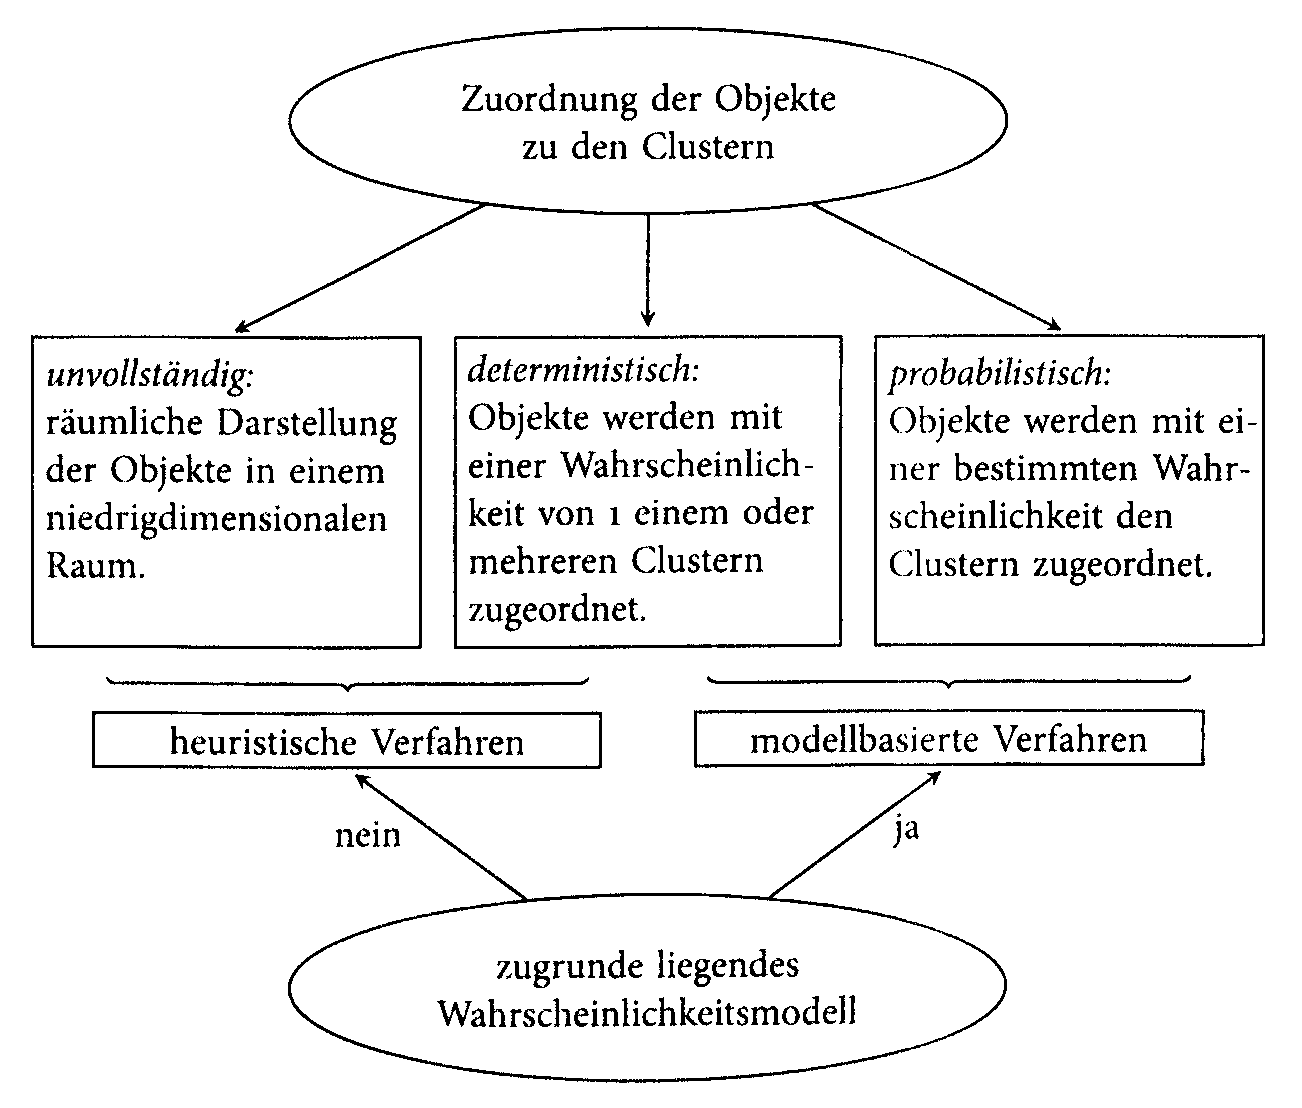
\includegraphics[width=10cm]{pics/bac20.png}
	\end{center}
	\caption{Wahrscheinlichkeitsmodelle nach Bacher et al.}
	\label{pic:bac20}
\end{figure}

Die partitionierenden Verfahren lassen sich wiederum in Austauschverfahren und iterierte Minimaldistanzverfahren unterscheiden.

\citet{Xu.1999} erwähnt weiterhin noch Single Scan Clustering, den BIRCH-Algorithmus, den STING-Algorithmus und Grid Clustering. Diese speziellen Algorithmen dienen der Klassifizierung bei räumlichen Datenbanken (Spatial Databases).